\documentclass{article}\usepackage[]{graphicx}\usepackage[]{color}
%% maxwidth is the original width if it is less than linewidth
%% otherwise use linewidth (to make sure the graphics do not exceed the margin)
\makeatletter
\def\maxwidth{ %
  \ifdim\Gin@nat@width>\linewidth
    \linewidth
  \else
    \Gin@nat@width
  \fi
}
\makeatother

\definecolor{fgcolor}{rgb}{0.345, 0.345, 0.345}
\newcommand{\hlnum}[1]{\textcolor[rgb]{0.686,0.059,0.569}{#1}}%
\newcommand{\hlstr}[1]{\textcolor[rgb]{0.192,0.494,0.8}{#1}}%
\newcommand{\hlcom}[1]{\textcolor[rgb]{0.678,0.584,0.686}{\textit{#1}}}%
\newcommand{\hlopt}[1]{\textcolor[rgb]{0,0,0}{#1}}%
\newcommand{\hlstd}[1]{\textcolor[rgb]{0.345,0.345,0.345}{#1}}%
\newcommand{\hlkwa}[1]{\textcolor[rgb]{0.161,0.373,0.58}{\textbf{#1}}}%
\newcommand{\hlkwb}[1]{\textcolor[rgb]{0.69,0.353,0.396}{#1}}%
\newcommand{\hlkwc}[1]{\textcolor[rgb]{0.333,0.667,0.333}{#1}}%
\newcommand{\hlkwd}[1]{\textcolor[rgb]{0.737,0.353,0.396}{\textbf{#1}}}%

\usepackage{framed}
\makeatletter
\newenvironment{kframe}{%
 \def\at@end@of@kframe{}%
 \ifinner\ifhmode%
  \def\at@end@of@kframe{\end{minipage}}%
  \begin{minipage}{\columnwidth}%
 \fi\fi%
 \def\FrameCommand##1{\hskip\@totalleftmargin \hskip-\fboxsep
 \colorbox{shadecolor}{##1}\hskip-\fboxsep
     % There is no \\@totalrightmargin, so:
     \hskip-\linewidth \hskip-\@totalleftmargin \hskip\columnwidth}%
 \MakeFramed {\advance\hsize-\width
   \@totalleftmargin\z@ \linewidth\hsize
   \@setminipage}}%
 {\par\unskip\endMakeFramed%
 \at@end@of@kframe}
\makeatother

\definecolor{shadecolor}{rgb}{.97, .97, .97}
\definecolor{messagecolor}{rgb}{0, 0, 0}
\definecolor{warningcolor}{rgb}{1, 0, 1}
\definecolor{errorcolor}{rgb}{1, 0, 0}
\newenvironment{knitrout}{}{} % an empty environment to be redefined in TeX

\usepackage{alltt}
\usepackage{amscd, amssymb, amsmath, verbatim, setspace}
\usepackage[left=1.0in, right=1.0in, top=1.0in, bottom=1.0in]{geometry}
\usepackage{mathrsfs}
\usepackage{listings}


\IfFileExists{upquote.sty}{\usepackage{upquote}}{}
\begin{document}
\begin{flushright}
Arif Ali\\
Math 611 Stochastic Simulation\\
Sept 8, 2016\\
\end{flushright}

\begin{center}
\LARGE\textbf{Homework 1}
  \end{center}
\section*{Exercise 1}
Let $U \sim Unif(0,1)$ and $X = g(u) = -c*ln(u)$ given that $c>0$
\begin{equation}
\begin{split}
X = -c*ln(U) \implies \\
-\frac{X}{c} = ln(U) \implies \\
e^{-\frac{X}{c}} = U \\
\therefore g^{-1}(u) = e^{-\frac{u}{c}}
\end{split}
\end{equation}

Since $U \sim Unif(0,1)$ the pdf is $f_U(u) = \frac{1}{1-0}=1$
In order to get the the pdf of X, the following is done:
\begin{equation}
\begin{split}
f(x)= f_U(g^{-1}(x))*\big|d/dx(g^{-1}(x)\big| = \\
1*\big|d/dx(e^{-x/c})\big| = \\
1*\big|-1/c*e^{-x/c}\big| =\\
1/c*e^{-x/c}\sim exp(1/c)
\end{split}
\end{equation}


\section*{Exercise 2}

\section*{Exercise 3}
\subsection*{Part A}

Let $z = 1+e^{-(x-\mu)/\beta} \implies dz = -\frac{1}{\beta}e^{-(x-\mu)/\beta}*dx \implies dx = \frac{dz}{-\frac{1}{\beta}e^{-(x-\mu)/\beta}}$
\begin{equation}
\begin{split}
F(x) = \int^{x}_{-\infty} f(x) dx = \\
\int\frac{1}{\beta}\frac{e^{-(x-\mu)/\beta}}{(1+e^{-(x-\mu)/\beta})^2}dx= \\
\int\frac{1}{\beta}\frac{e^{-(x-\mu)/\beta}}{z^2}*\frac{dz}{-\frac{1}{\beta}e^{-(x-\mu)/\beta}}= \\
\int-\frac{1}{z^2}dz= \\
\frac{1}{z}=\big|^{x}_{-\infty}\frac{1}{1+e^{-(x-\mu)/\beta}}=\frac{1}{1+e^{-(x-\mu)/\beta}}
\end{split}
\end{equation}

To find the inverse, we do the following:
\begin{equation}
\begin{split}
Y = \frac{1}{1+e^{-(x-\mu)/\beta}} \implies\\
1+e^{-(x-\mu)/\beta} = \frac{1}{Y} \implies\\
e^{-(x-\mu)/\beta} = \frac{1}{Y} - 1 \implies\\
-(x-\mu)/\beta = ln(\frac{1}{Y} - 1) \implies\\
-(x-\mu) = ln(\frac{1}{Y} - 1)\beta \implies\\
x = \mu - ln(\frac{1}{Y} - 1)\beta
\therefore F^{-1}(x) = \mu - ln(\frac{1}{x} - 1)\beta
\end{split}
\end{equation}
\begin{knitrout}
\definecolor{shadecolor}{rgb}{0.969, 0.969, 0.969}\color{fgcolor}\begin{kframe}
\begin{alltt}
\hlstd{u} \hlkwb{=} \hlkwd{runif}\hlstd{(}\hlnum{1e4}\hlstd{)}

\hlstd{inverse_logistic_cdf} \hlkwb{=} \hlkwa{function}\hlstd{(}\hlkwc{x}\hlstd{,} \hlkwc{mu} \hlstd{=} \hlnum{0} \hlstd{,} \hlkwc{B} \hlstd{=} \hlnum{1}\hlstd{)\{}
  \hlstd{mu} \hlopt{-} \hlkwd{log}\hlstd{(}\hlnum{1}\hlopt{/}\hlstd{x}\hlopt{-}\hlnum{1}\hlstd{)}\hlopt{*}\hlstd{B}
\hlstd{\}}

\hlstd{it_logistic} \hlkwb{=} \hlkwd{inverse_logistic_cdf}\hlstd{(u)}
\hlstd{r_logistic} \hlkwb{=} \hlkwd{rlogis}\hlstd{(}\hlnum{1e4}\hlstd{)}

\hlkwd{hist}\hlstd{(it_logistic,} \hlkwc{breaks} \hlstd{=} \hlnum{50}\hlstd{,} \hlkwc{col} \hlstd{=} \hlstr{"green"}\hlstd{)}
\hlkwd{hist}\hlstd{(r_logistic,} \hlkwc{breaks} \hlstd{=} \hlnum{50}\hlstd{,} \hlkwc{col} \hlstd{=} \hlstr{"#FF000099"}\hlstd{,} \hlkwc{add} \hlstd{= T)}
\end{alltt}
\end{kframe}
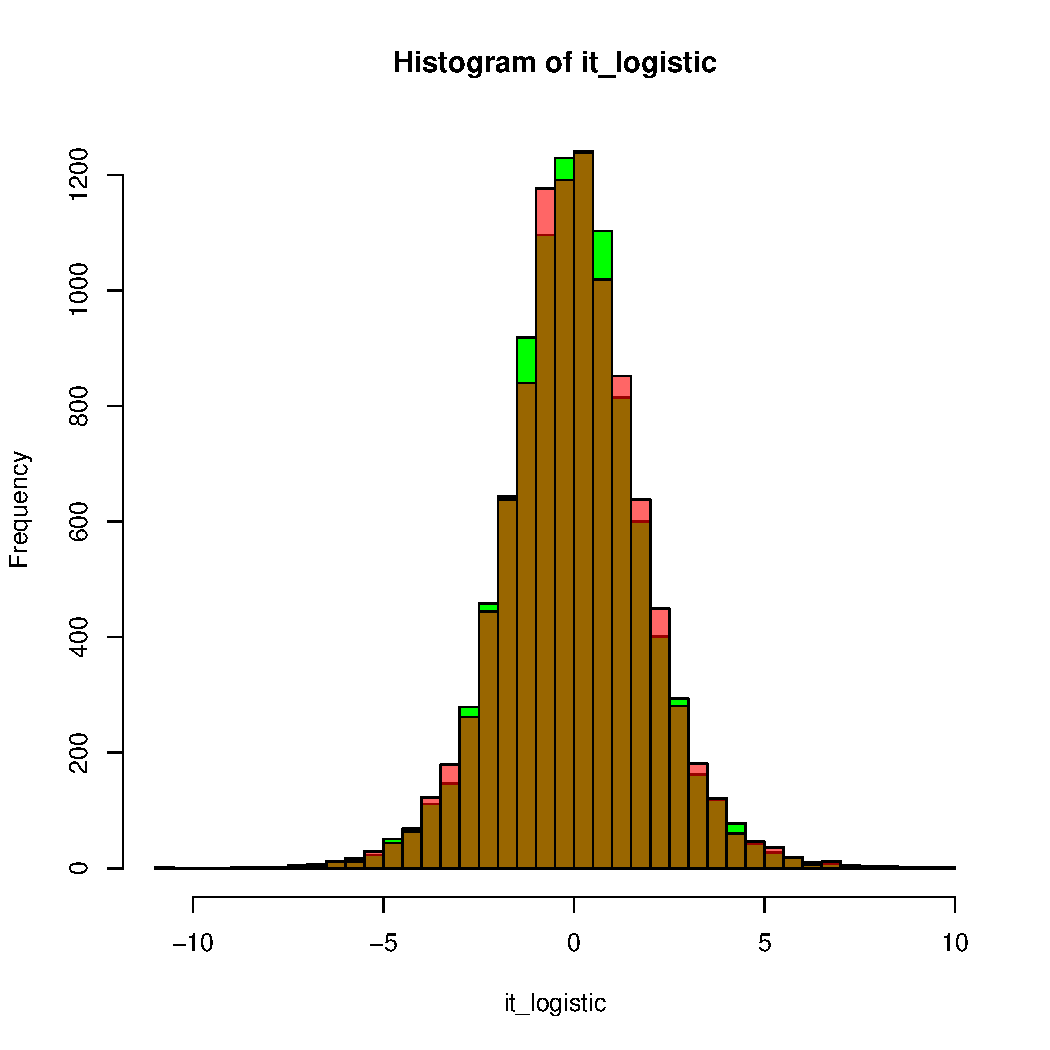
\includegraphics[width=0.50\linewidth]{figure/unnamed-chunk-2-1} 

\end{knitrout}
Based on a comparision of the histograms of the sampled inverse function of the logistic distribution against the random generator of the logistic distribution, their seems to be a close relationship between the two. This indicates a similar behavior, which could lead to the conclusion that both functions act in the the same way. 

\subsection*{Part B}
Let $tan(z)=\frac{x-\mu}{\sigma}\implies dz*sec^{2}(z)=\frac{1}{\sigma}*dx \implies dx = \sigma * sec^{2}(z)*dz$
\begin{equation}
\begin{split}
F(x) = \int^{x}_{-\infty} f(x) dx = \\
\int \frac{1}{\pi*\sigma}*\frac{1}{1+(\frac{x-\mu}{\sigma})^2}dx = \\
\int \frac{1}{\pi*\sigma}*\frac{1}{1+tan^2(z)}*\sigma * sec^{2}(z)*dz = \\
\frac{1}{\pi} \int 1 *dz = \\
\frac{1}{\pi} \big|z = \\
\frac{1}{\pi} \big|^{x}_{-\infty}arctan(\frac{x-\mu}{\sigma}) = \\
\frac{1}{\pi}*arctan(\frac{x-\mu}{\sigma})+\frac{1}{2}
\end{split}
\end{equation}
To find the inverse, we do the following:
\begin{equation}
\begin{split}
\frac{1}{\pi}*arctan(\frac{x-\mu}{\sigma})+\frac{1}{2} = Y \implies \\
\pi*(Y-\frac{1}{2} = arctan(\frac{x-\mu}{\sigma})) \implies
tan(\pi*(Y-\frac{1}{2})) = \frac{x-\mu}{\sigma} \implies \\
\sigma*tan(\pi*(Y-\frac{1}{2})) + \mu = x \\
\therefore F^{-1}(x) = \sigma*tan(\pi*(x-\frac{1}{2})) + \mu
\end{split}
\end{equation}
\begin{knitrout}
\definecolor{shadecolor}{rgb}{0.969, 0.969, 0.969}\color{fgcolor}\begin{kframe}
\begin{alltt}
\hlstd{inverse_cauchy_cdf} \hlkwb{=} \hlkwa{function}\hlstd{(}\hlkwc{x}\hlstd{,} \hlkwc{mu} \hlstd{=} \hlnum{0}\hlstd{,} \hlkwc{sigma} \hlstd{=} \hlnum{1}\hlstd{)\{}
  \hlstd{sigma}\hlopt{*}\hlkwd{tan}\hlstd{(pi}\hlopt{*}\hlstd{(x}\hlopt{-}\hlnum{0.5}\hlstd{))} \hlopt{+} \hlstd{mu}
\hlstd{\}}
\hlstd{u} \hlkwb{=} \hlkwd{runif}\hlstd{(}\hlnum{1e4}\hlstd{)}
\hlstd{it_cauchy} \hlkwb{=} \hlkwd{inverse_cauchy_cdf}\hlstd{(u)}
\hlstd{r_cauchy} \hlkwb{=} \hlkwd{rcauchy}\hlstd{(}\hlnum{1e4}\hlstd{)}


\hlkwd{hist}\hlstd{(it_cauchy,} \hlkwc{breaks} \hlstd{=} \hlnum{50}\hlstd{,} \hlkwc{col} \hlstd{=} \hlstr{"blue"}\hlstd{)}
\hlkwd{hist}\hlstd{(r_cauchy,} \hlkwc{breaks} \hlstd{=} \hlnum{50}\hlstd{,} \hlkwc{col} \hlstd{=} \hlstr{"#FF000099"}\hlstd{,} \hlkwc{add} \hlstd{= T)}
\end{alltt}
\end{kframe}
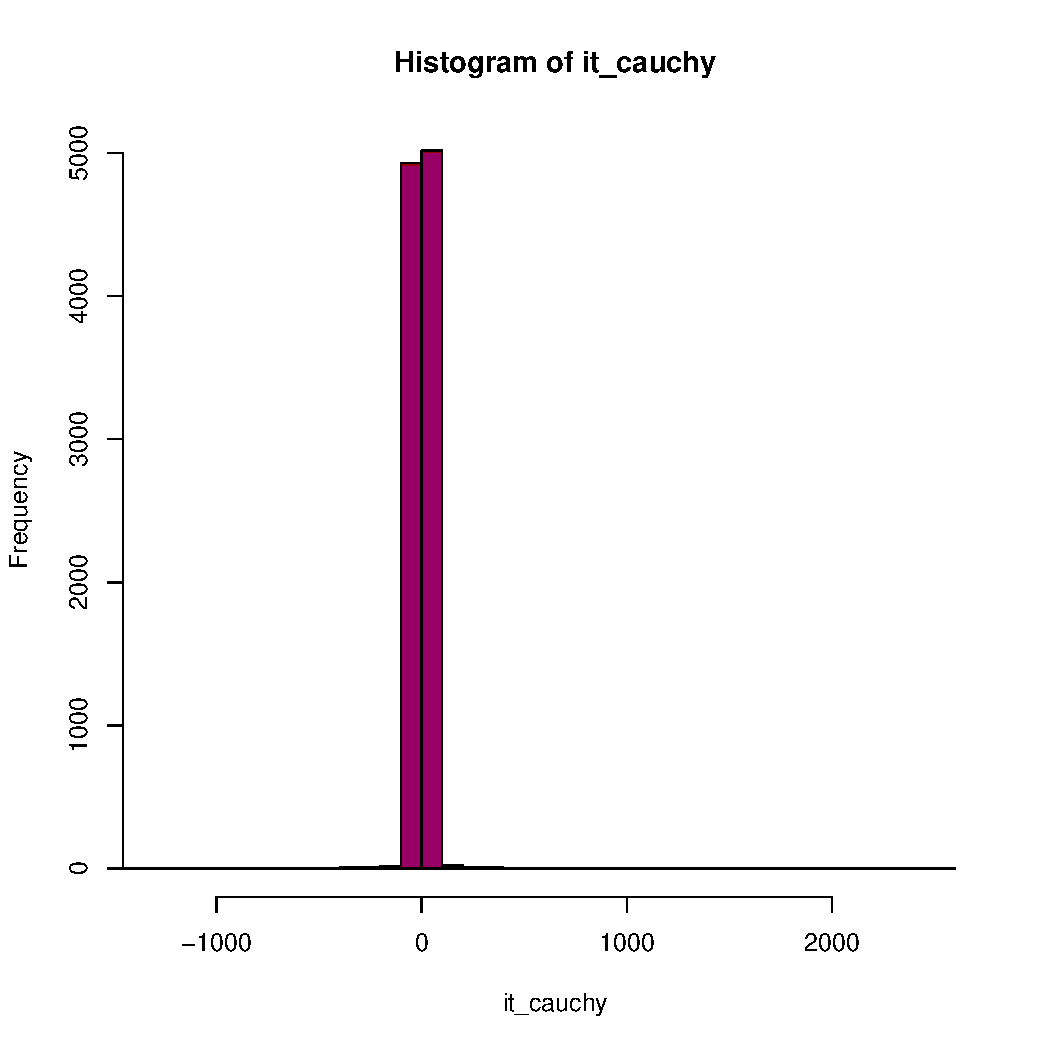
\includegraphics[width=0.50\linewidth]{figure/unnamed-chunk-3-1} 

\end{knitrout}
In both cases, the cauchy distribution seems to settle on numbers close to 0. However, the tails are harder to compare. Since there seems to be an overlap with the majority of points, it may be concluded that the inverse of the cauchy distribution act similar to the random generated sample of the cauchy distribution.

John Hotchkiss recommended looking at the density plot and qqplots between the two samples
\begin{knitrout}
\definecolor{shadecolor}{rgb}{0.969, 0.969, 0.969}\color{fgcolor}\begin{kframe}
\begin{alltt}
\hlkwd{par}\hlstd{(}\hlkwc{mfrow}\hlstd{=}\hlkwd{c}\hlstd{(}\hlnum{1}\hlstd{,}\hlnum{2}\hlstd{))}
\hlkwd{qqplot}\hlstd{(it_cauchy, r_cauchy)}
\hlkwd{plot}\hlstd{(}\hlkwd{density}\hlstd{(it_cauchy))}
\hlkwd{lines}\hlstd{(}\hlkwd{density}\hlstd{(r_cauchy),} \hlkwc{col} \hlstd{=} \hlstr{"red"}\hlstd{)}
\end{alltt}
\end{kframe}
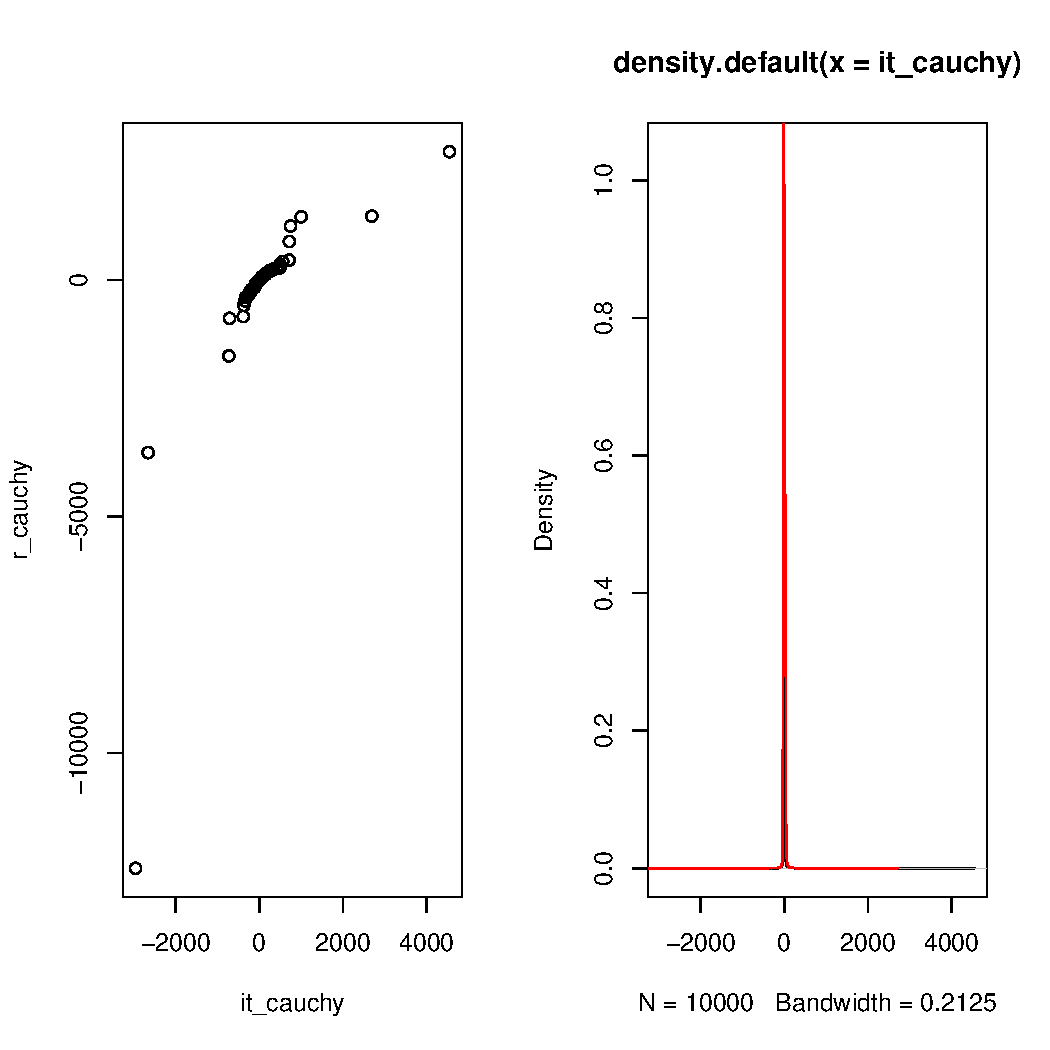
\includegraphics[width=0.50\linewidth]{figure/unnamed-chunk-4-1} 

\end{knitrout}
The qqplot doesn't show a clear relationship between the the two, but the density plot shows a convergence at 0 for both densities

\section*{Exercise 4}
\begin{knitrout}
\definecolor{shadecolor}{rgb}{0.969, 0.969, 0.969}\color{fgcolor}\begin{kframe}
\begin{alltt}
\hlkwd{par}\hlstd{(}\hlkwc{mfrow}\hlstd{=}\hlkwd{c}\hlstd{(}\hlnum{1}\hlstd{,}\hlnum{2}\hlstd{))}
\hlstd{u1} \hlkwb{=} \hlkwd{runif}\hlstd{(}\hlnum{1e3}\hlstd{)}
\hlstd{u2} \hlkwb{=} \hlkwd{runif}\hlstd{(}\hlnum{1e3}\hlstd{)}

\hlstd{z1} \hlkwb{=} \hlkwd{sqrt}\hlstd{(}\hlopt{-}\hlnum{2}\hlopt{*}\hlkwd{log}\hlstd{(u1))}\hlopt{*}\hlkwd{cos}\hlstd{(}\hlnum{2}\hlopt{*}\hlstd{pi}\hlopt{*}\hlstd{u2)}
\hlstd{z2} \hlkwb{=} \hlkwd{sqrt}\hlstd{(}\hlopt{-}\hlnum{2}\hlopt{*}\hlkwd{log}\hlstd{(u1))}\hlopt{*}\hlkwd{sin}\hlstd{(}\hlnum{2}\hlopt{*}\hlstd{pi}\hlopt{*}\hlstd{u2)}


\hlkwd{qqnorm}\hlstd{(z1)}
\hlkwd{qqline}\hlstd{(z1,} \hlkwc{col} \hlstd{=} \hlstr{"red"}\hlstd{)}
\hlkwd{plot}\hlstd{(}\hlkwd{density}\hlstd{(z1))}
\hlkwd{lines}\hlstd{(}\hlkwd{seq}\hlstd{(}\hlkwd{min}\hlstd{(z1),}\hlkwd{max}\hlstd{(z1),} \hlkwc{length} \hlstd{=} \hlnum{1e4}\hlstd{),} \hlkwd{dnorm}\hlstd{(}\hlkwd{seq}\hlstd{(}\hlkwd{min}\hlstd{(z1),}\hlkwd{max}\hlstd{(z1),} \hlkwc{length} \hlstd{=} \hlnum{1e4}\hlstd{)),} \hlkwc{col} \hlstd{=} \hlstr{"red"}\hlstd{)}
\end{alltt}
\end{kframe}
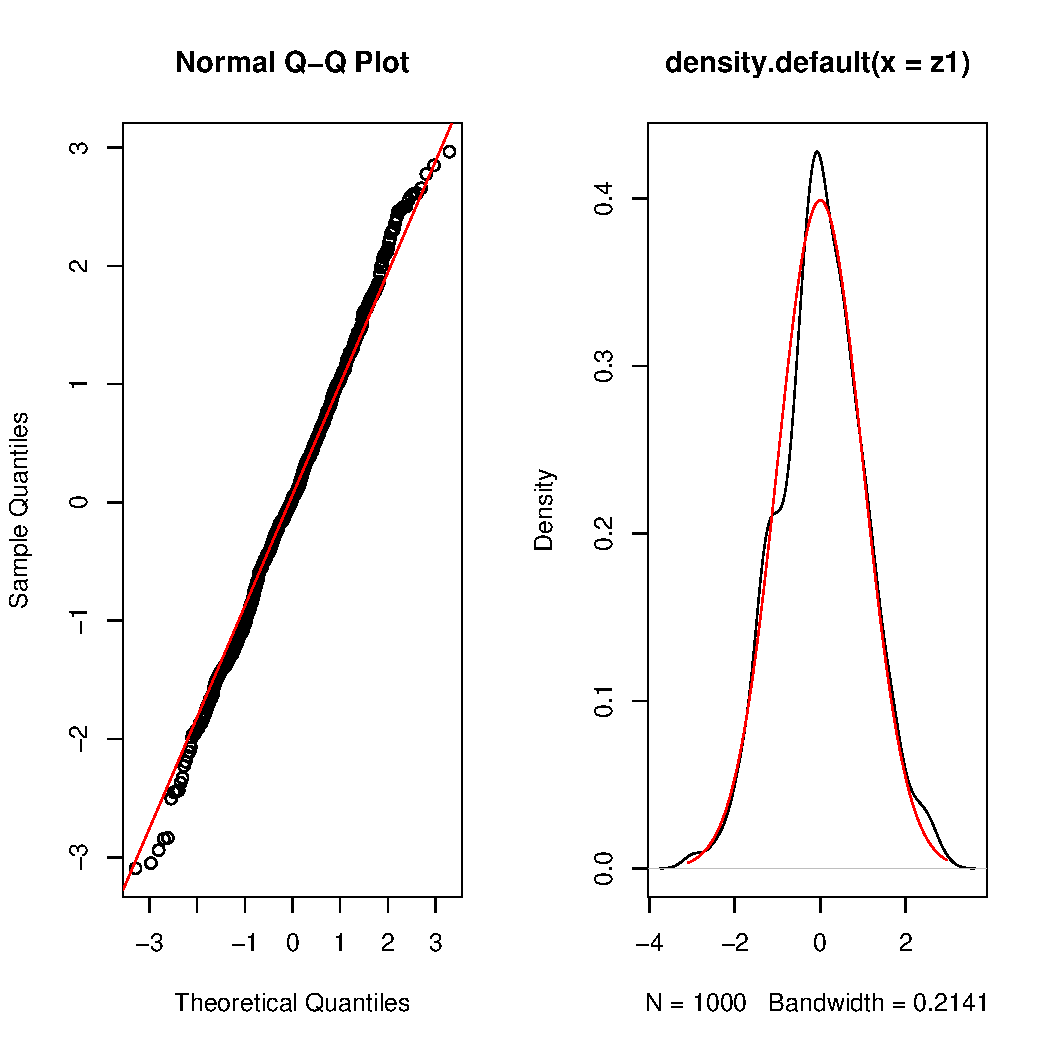
\includegraphics[width=0.50\linewidth]{figure/unnamed-chunk-5-1} 
\begin{kframe}\begin{alltt}
\hlkwd{qqnorm}\hlstd{(z2)}
\hlkwd{qqline}\hlstd{(z2,} \hlkwc{col} \hlstd{=} \hlstr{"red"}\hlstd{)}
\hlkwd{plot}\hlstd{(}\hlkwd{density}\hlstd{(z2))}
\hlkwd{lines}\hlstd{(}\hlkwd{seq}\hlstd{(}\hlkwd{min}\hlstd{(z2),}\hlkwd{max}\hlstd{(z2),} \hlkwc{length} \hlstd{=} \hlnum{1e4}\hlstd{),} \hlkwd{dnorm}\hlstd{(}\hlkwd{seq}\hlstd{(}\hlkwd{min}\hlstd{(z1),}\hlkwd{max}\hlstd{(z1),} \hlkwc{length} \hlstd{=} \hlnum{1e4}\hlstd{)),} \hlkwc{col} \hlstd{=} \hlstr{"red"}\hlstd{)}
\end{alltt}
\end{kframe}
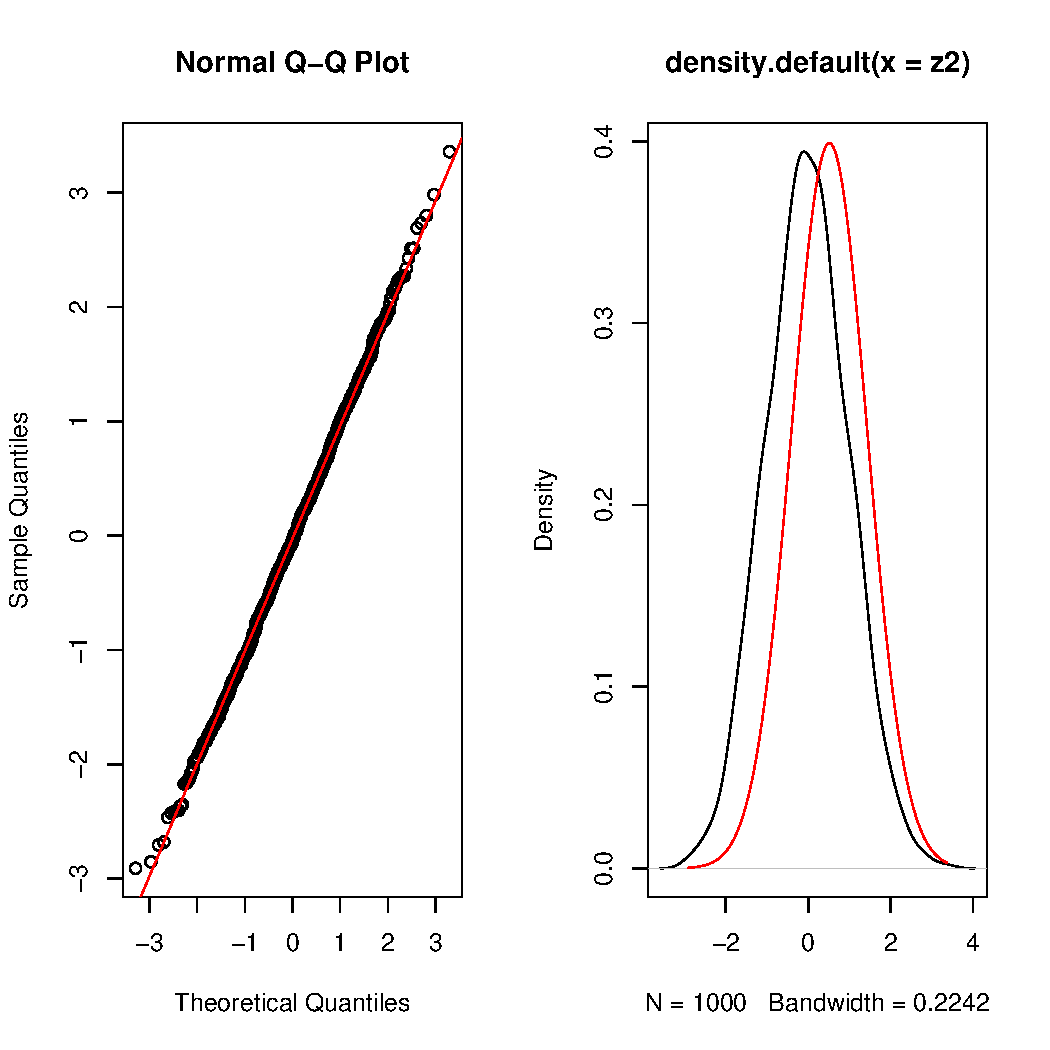
\includegraphics[width=0.50\linewidth]{figure/unnamed-chunk-5-2} 

\end{knitrout}
Both $Z_1$ and $Z_2$ follow a normal distribution based on a comparison of plots with the normal distribution's density along with the qqplots against the normal distribution. 
\section*{Exercise 5}
To Prove CLT works for a non-normal distribution, the beta distribution was sampled with $\alpha = 1$ and $\beta=2$ such that $Samples \sim beta(1,2)$
\begin{knitrout}
\definecolor{shadecolor}{rgb}{0.969, 0.969, 0.969}\color{fgcolor}\begin{kframe}
\begin{alltt}
\hlstd{samples} \hlkwb{=} \hlkwd{matrix}\hlstd{(}\hlkwc{nrow} \hlstd{=} \hlnum{35}\hlstd{,} \hlkwc{ncol} \hlstd{=} \hlnum{1e3}\hlstd{)}
\hlkwa{for}\hlstd{(i} \hlkwa{in} \hlnum{1}\hlopt{:}\hlnum{1000}\hlstd{)\{}
  \hlstd{samples[,i]} \hlkwb{=} \hlkwd{rbeta}\hlstd{(}\hlnum{35}\hlstd{,} \hlnum{1}\hlstd{,}\hlnum{2}\hlstd{)}
\hlstd{\}}
\end{alltt}
\end{kframe}
\end{knitrout}
\subsection*{Part A}
\begin{knitrout}
\definecolor{shadecolor}{rgb}{0.969, 0.969, 0.969}\color{fgcolor}\begin{kframe}
\begin{alltt}
\hlstd{means} \hlkwb{=} \hlkwd{apply}\hlstd{(samples,} \hlnum{2}\hlstd{, mean)}
\hlkwd{summary}\hlstd{(means)}
\end{alltt}
\begin{verbatim}
##    Min. 1st Qu.  Median    Mean 3rd Qu.    Max. 
##  0.2180  0.3041  0.3289  0.3310  0.3575  0.4604
\end{verbatim}
\begin{alltt}
\hlkwd{sd}\hlstd{(means)}
\end{alltt}
\begin{verbatim}
## [1] 0.03963573
\end{verbatim}
\end{kframe}
\end{knitrout}
From the definition of the beta distribution, $E(X) = \frac{\alpha}{\alpha+\beta}=\frac{1}{1+2}=\frac{1}{3}$
Based on the summary, the mean that is approximated is very close to the theortical mean.

The variance is defined as $Var(X)=\frac{\alpha*\beta}{(\alpha+\beta)^2*(\alpha+\beta+1)}$ Since we are dealing with a sample of $n=35$, the standard deviation should be $SD(X)=\sqrt{\frac{\alpha*\beta}{(\alpha+\beta)^2*(\alpha+\beta+1)}/35}= 0.0398$. The approximated value is also close to the theortical standard deviation.

\subsection*{Part B}
\begin{knitrout}
\definecolor{shadecolor}{rgb}{0.969, 0.969, 0.969}\color{fgcolor}\begin{kframe}
\begin{alltt}
\hlkwd{qqnorm}\hlstd{(means)}
\hlkwd{qqline}\hlstd{(means,} \hlkwc{col} \hlstd{=} \hlstr{"red"}\hlstd{)}
\end{alltt}
\end{kframe}
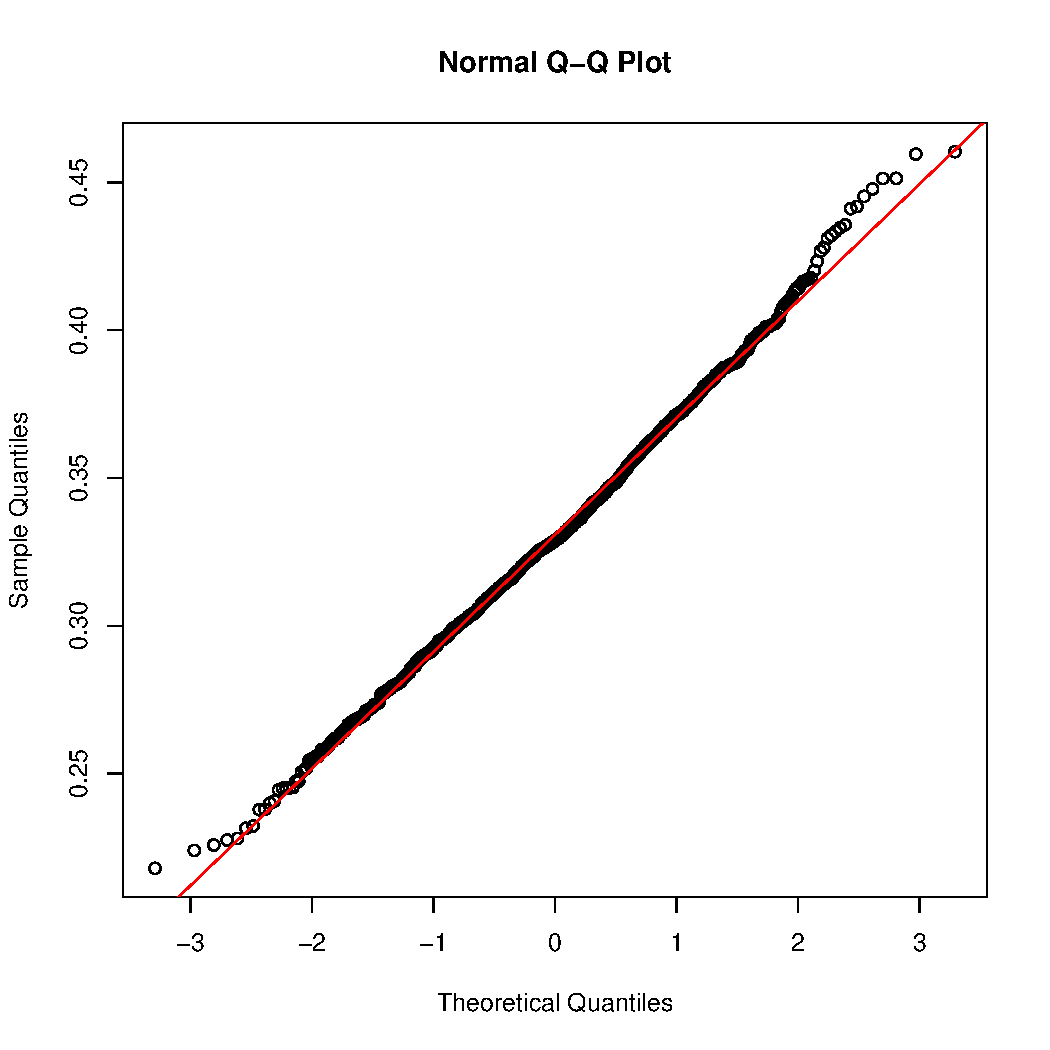
\includegraphics[width=0.50\linewidth]{figure/unnamed-chunk-8-1} 

\end{knitrout}
Based off the qqplot, the distribution of means follows closely to the normal distribution; however, there are some noticable movements away from the qqline at the tail ends. 
\end{document}
